\chapter{Ergebnisse} \label{sec:results}

Das Kapitel stellt die Ergebnisse der Tests der verschiedenen Modelle dar. Außerdem 
wird eine Übersicht über die benötigte Trainingszeit für die Modelle gegeben. 

\section{Benötigte Trainingszeit}

\begin{itemize}
    \item Eine Epoche des Pre-Trainings auf dem Combined-Straßendatensatz dauert zwischen 40 und 50 Minuten. 
    \item Eine Epoche des Trainings auf dem BikeSat-Datensatz dauert zwischen 10 und 17 Minuten. 
    \item Die Netze konvergieren nach circa 33-57 Epochen auf beiden Datensätzen. 
    \item Das Training wird immer vorzeitig vor dem Ablaufen der 100 Epochen beendet.
    \item Der zeitliche Mehraufwand durch die Bild-Augmentierung während des Trainings (vgl. \autoref{sec:pre-processing}) 
    liegt im Schnitt bei 3 min 30s pro Epoche für beide Augmentierungsmethoden (Basic-Augmentation und Color-Augmentation).  
\end{itemize}

\section{Pre-Training-Ergebnisse zur Straßenerkennung}

\begin{table}[ht]
	\centering
	\begin{tabular}{l|c|c}
		Modell & \ac{IoU} & \ac{BIoU} \\
		\midrule
        BUNet2 & 57,13 & 76,71 \\ 
        BUNet15 & 60,75 & 80,80 \\ 
        VBUNet & \textbf{64,26} & \textbf{85,64} \\ 
        RBUNet & 61,45 & 83,86 \\ 
        DBUNet & 62,56 & 84,46 \\ 
        
	\end{tabular}
	\caption{Ergebnisse des Pre-Trainings der Modelle auf der Testpartition des Combined-Datensatzes in Prozent.}
	\label{tab:results-roads}
\end{table}

\begin{figure}
	\centering
	\begin{minipage}{.41\textwidth}
		\centering
		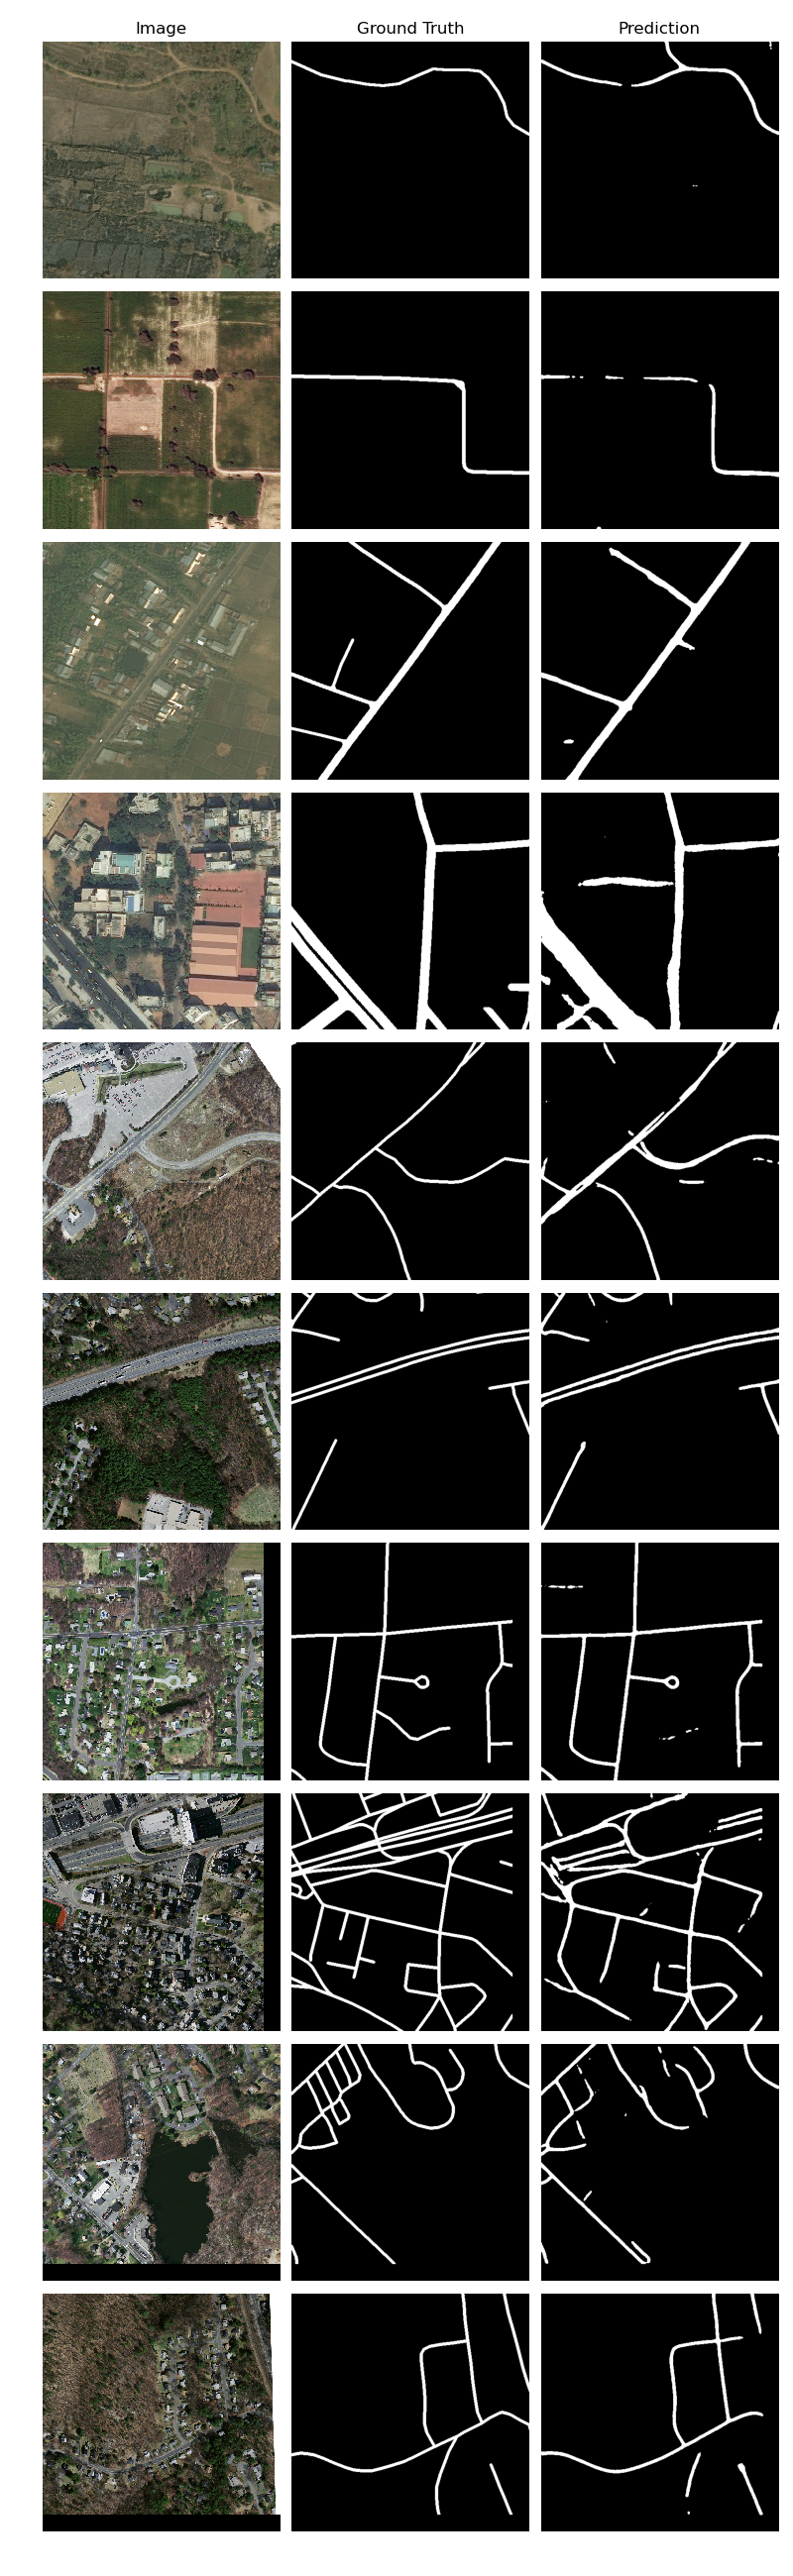
\includegraphics[width=1.\linewidth]{Bilder/Samples-Combined/bunet2.png}
	\end{minipage}
	\begin{minipage}{.41\textwidth}
		\centering
		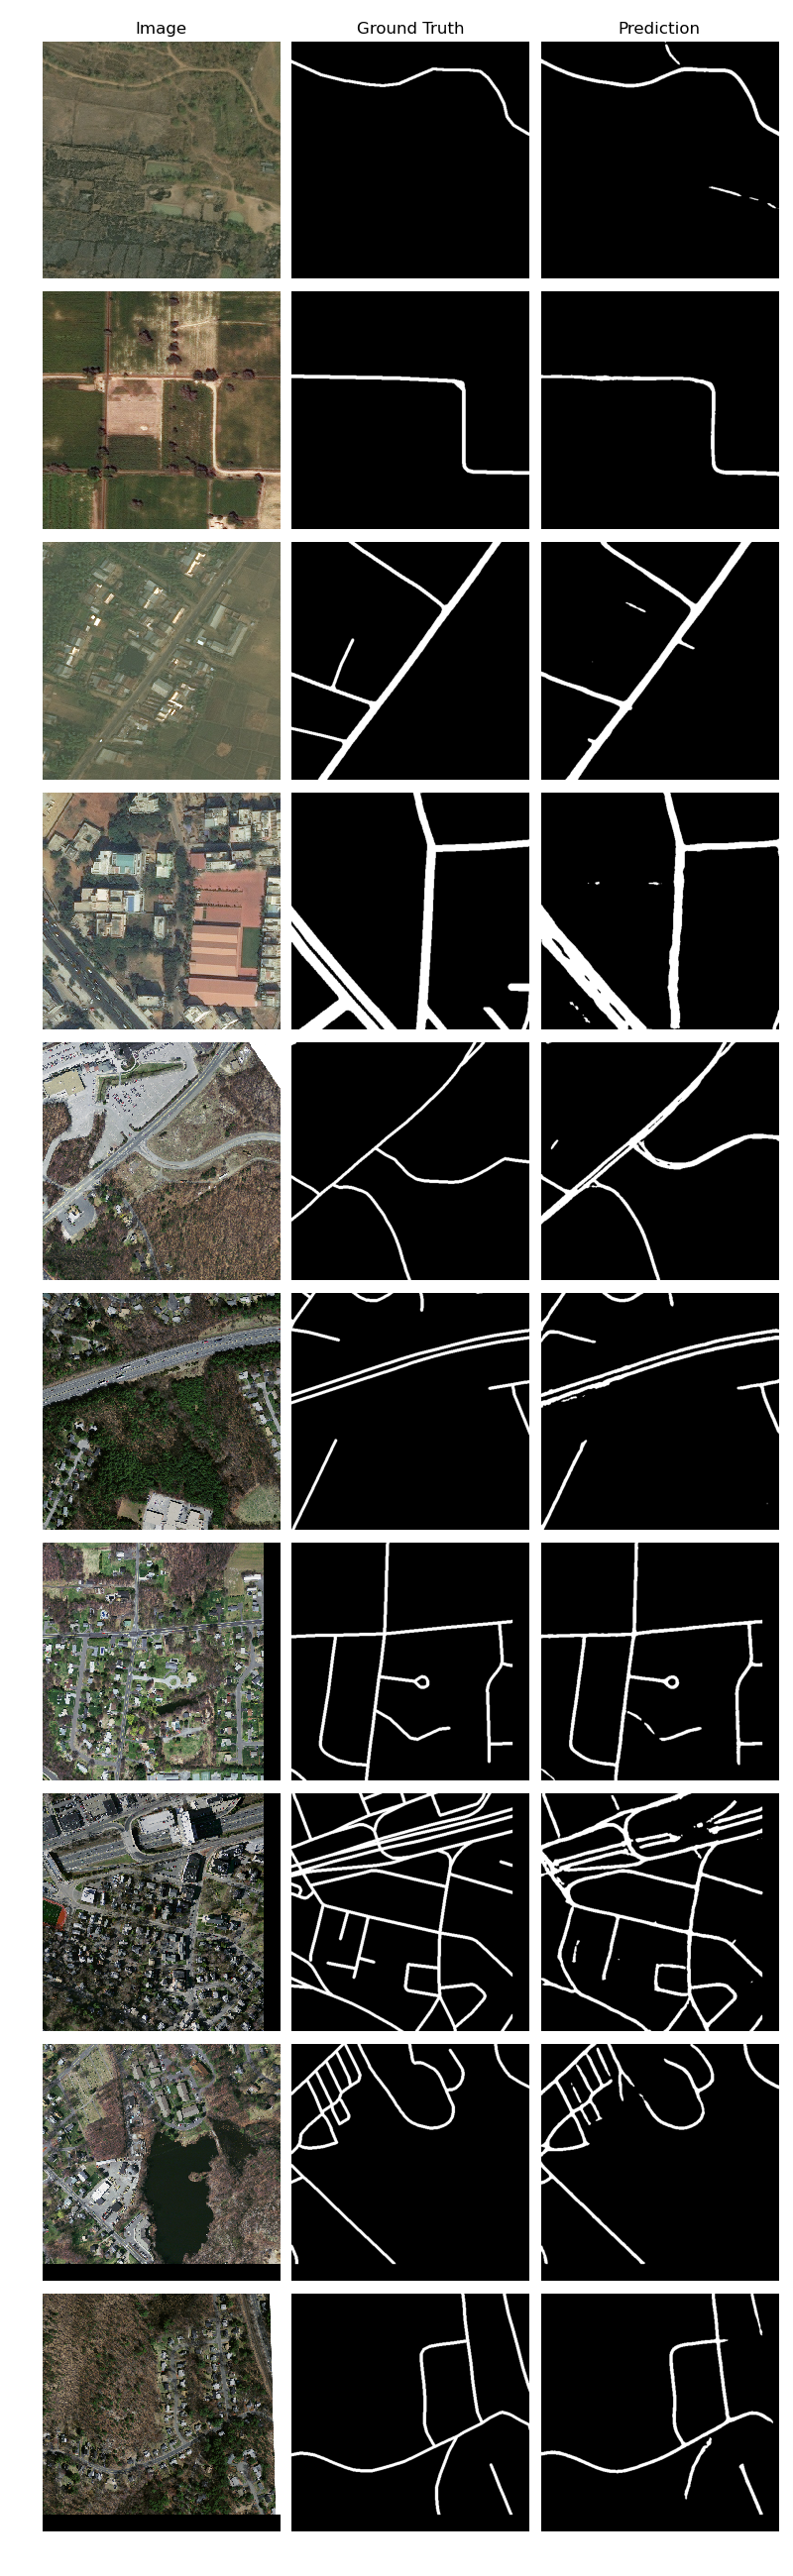
\includegraphics[width=1.\linewidth]{Bilder/Samples-Combined/vbunet.png}
	\end{minipage}

	\caption{Beispiel-Predictions des $BUNet2$ (links) und $VBUNet$ (rechts) auf dem Combined-Datensatz.}
	\label{fig:combined-samples-bune2-vbunet}
\end{figure}

\autoref{tab:results-roads} zeigt die Test-Ergebnisse der Modelle nach Training auf dem Combined-Datensatz 
(vgl. \autoref{sec:pre-training-roads}) in Prozent. Pro Spalte ist das höchste Ergebnis hervorgehoben. 
\ac{BUNet2} und \ac{BUNet15} sind von Grund auf trainiert, während \ac{VBUNet}, \ac{RBUNet} und \ac{DBUNet} einen auf 
ImageNet vortrainierten Encoder aufweisen. Die \ac{BIoU} verwendet wie bei der Radwegerkennung und wie in \autoref{sec:eval:biou} 
festgelegt eine Puffergröße von 15 Pixeln. 

\autoref{fig:combined-samples-bune2-vbunet} zeigt ausgewählte Beispielpredictions des \ac{BUNet2} (links) und 
des \ac{VBUNet}.\footnote{Weitere Beispiele anderer Netze in \autoref{sec:pred-combined}.}

\section{Ergebnisse der Radwegerkennung}

\begin{table}[ht]
	\centering
	\begin{tabular}{l|cc|cc|cc|cc}
		& \multicolumn{4}{c|}{Basic Augmentation} & \multicolumn{4}{c}{Color Augmentation} \\
        & \multicolumn{2}{c|}{BikeSat} & \multicolumn{2}{c|}{Karlsruhe} & \multicolumn{2}{c|}{BikeSat} & \multicolumn{2}{c}{Karlsruhe} \\
		Modell & \ac{IoU} & \ac{BIoU} & \ac{IoU} & \ac{BIoU} & \ac{IoU} & \ac{BIoU} & \ac{IoU} & \ac{BIoU} \\
		\midrule
        BUNet2$^*$ & 23,54 & 47,71 & 01,30 & 34,80 &  27,47 & 55,19 & 12,69 & 47,53 \\
        BUNet2$^l$ & 24,48 & 51,77 & 02,19 & 12,11 &  28,06 & 57,21 & 08,54 & 39,19 \\
        BUNet2$^r$ & 25,35 & 51,27 & 09,36 & 47,57 &  25,95 & 53,73 & 04,56 & 25,97 \\
		\midrule

        BUNet15$^*$ & 27,93 & 56,55 & \textbf{21,52} & \textbf{59,25} &  30,80 & 59,99 & 06,84 & 33,23 \\
        BUNet15$^l$ & 28,14 & 57,14 & 16,47 & 54,17 &  30,98 & 60,50 & 07,47 & 30,20 \\
        BUNet15$^r$ & 28,22 & 57,26 & 10,17 & 53,81 &  29,95 & 59,46 & 08,23 & 26,82 \\
		\midrule

        VBUNet$^*$ & 30,45 & 61,48 & 09,69 & 37,84 &  \textbf{31,71} & \textbf{61,32} & 09,29 & 31,15 \\
        VBUNet$^l$ & \underline{\textbf{32,24}} & \textbf{62,93} & 12,85 & 54,91 &  21,91 & 45,88 & 03,19 & 23,25 \\
        VBUNet$^r$ & \textbf{31,84} & 61,51 & 17,53 & \textbf{61,51} &  25,65 & 51,82 & 10,74 & 32,31 \\
		\midrule

        RBUNet$^*$ & 29,11 & 60,53 & 11,74 & 32,80 &  \underline{\textbf{33,54}} & \underline{\textbf{65,02}} & \textbf{23,24} & \textbf{65,71} \\
        RBUNet$^l$ & 30,98 & 60,51 & \underline{\textbf{24,67}} & \underline{\textbf{65,27}} &  29,32 & 59,83 & 09,67 & 53,08 \\
        RBUNet$^r$ & 31,31 & \underline{\textbf{63,55}} & \textbf{18,21} & 55,53 &  29,42 & 59,58 & \underline{\textbf{34,66}} & \underline{\textbf{68,26}} \\
		\midrule

        DBUNet$^*$ & 30,76 & 61,78 & 07,14 & 45,97 &  \textbf{32,24} & \textbf{64,77} & 14,64 & 50,02 \\
        DBUNet$^l$ & 31,55 & 62,38 & 17,47 & 55,20 &  29,64 & 60,47 & 14,83 & 51,19 \\
        DBUNet$^r$ & \textbf{32,12} & \textbf{62,99} & 14,03 & 51,73 &  30,30 & 61,24 & 17,43 & \textbf{62,28} \\
        
	\end{tabular}
	\caption{Ergebnisse der Modelle auf der Testpartition des BikeSat-Datensatzes und dem Karlsruhe-Datensatz
	für beide Augmentierungsmethoden. 
    In Prozent.}
	\label{tab:results}
\end{table}

\autoref{tab:results} zeigt die Test-Ergebnisse der Modelle nach Training (s. \autoref{sec:training} für Details) auf dem BikeSat-Datensatz 
(s. \autoref{sec:bike-data}) für jede Augmentierungsmethode (Basic- u. Color-Augmentation) während des Trainings in Prozent. 
Zusätzlich zeigt die Tabelle die Test-Ergebnisse auf allen 196 $512{\times}512$-Ausschnitten 
des Karlsruhe-Datensatz (s. \autoref{sec:karlsruhe}) in Prozent. Der Karlsruhe-Datensatz in dieser Tabelle
enthält auch Ausschnitte, die \textit{keine} Radwege enthalten. \\ 
Pro Spalte sind die höchsten drei Ergebnisse hervorgehoben und das höchste unterstrichen.
Die \ac{BIoU} hat eine Puffergröße von 15 Pixeln, wie in \autoref{sec:eval:biou} festgelegt.\\


\begin{table}[ht]
	\centering
	\begin{tabular}{l|cc|cc|cc}
        & \multicolumn{2}{c|}{\textcolor{gray}{BikeSat}} & \multicolumn{2}{c|}{\textcolor{gray}{Karlsruhe}} & \multicolumn{2}{c}{Wolfsburg} \\
		Modell & \textcolor{gray}{\ac{IoU}} & \textcolor{gray}{\ac{BIoU}} & \textcolor{gray}{\ac{IoU}} & \textcolor{gray}{\ac{BIoU}} & \ac{IoU} & \ac{BIoU} \\
		\midrule
        BUNet2$^*$ & \textcolor{gray}{27,47} & \textcolor{gray}{55,19} & \textcolor{gray}{12,69} & \textcolor{gray}{47,53} &  28,44 & 57,30 \\
        BUNet2$^l$ & \textcolor{gray}{28,06} & \textcolor{gray}{57,21} & \textcolor{gray}{08,54} & \textcolor{gray}{39,19} &  29,92 & 59,64 \\
        BUNet2$^r$ & \textcolor{gray}{25,95} & \textcolor{gray}{53,73} & \textcolor{gray}{04,56} & \textcolor{gray}{25,97} &  28,62 & 57,98 \\
		\midrule

        BUNet15$^*$ & \textcolor{gray}{30,80} & \textcolor{gray}{59,99} & \textcolor{gray}{06,84} & \textcolor{gray}{33,23} &  30,68 & 61,86 \\
        BUNet15$^l$ & \textcolor{gray}{30,98} & \textcolor{gray}{60,50} & \textcolor{gray}{07,47} & \textcolor{gray}{30,20} &  31,31 & 61,71 \\
        BUNet15$^r$ & \textcolor{gray}{29,95} & \textcolor{gray}{59,46} & \textcolor{gray}{08,23} & \textcolor{gray}{26,82} &  30,99 & 60,84 \\
		\midrule

        VBUNet$^*$ & \textcolor{gray}{\textbf{31,71}} & \textcolor{gray}{\textbf{61,32}} & \textcolor{gray}{09,29} & \textcolor{gray}{31,15} &  \textbf{32,90} & \textbf{66,08} \\
        VBUNet$^l$ & \textcolor{gray}{21,91} & \textcolor{gray}{45,88} & \textcolor{gray}{03,19} & \textcolor{gray}{23,25} &  22,79 & 50,18 \\
        VBUNet$^r$ & \textcolor{gray}{25,65} & \textcolor{gray}{51,82} & \textcolor{gray}{10,74} & \textcolor{gray}{32,31} &  27,53 & 56,97 \\
		\midrule

        RBUNet$^*$ & \textcolor{gray}{\underline{\textbf{33,54}}} & \textcolor{gray}{\underline{\textbf{65,02}}} & \textcolor{gray}{\textbf{23,24}} & \textcolor{gray}{\textbf{65,71}} &  \underline{\textbf{34,42}} & \textbf{67,74} \\
        RBUNet$^l$ & \textcolor{gray}{29,32} & \textcolor{gray}{59,83} & \textcolor{gray}{09,67} & \textcolor{gray}{53,08} &  30,80 & 63,30 \\
        RBUNet$^r$ & \textcolor{gray}{29,42} & \textcolor{gray}{59,58} & \textcolor{gray}{\underline{\textbf{34,66}}} & \textcolor{gray}{\underline{\textbf{68,26}}} &  31,17 & 63,47 \\
		\midrule

        DBUNet$^*$ & \textcolor{gray}{\textbf{32,24}} & \textcolor{gray}{\textbf{64,77}} & \textcolor{gray}{14,64} & \textcolor{gray}{50,02} &  \textbf{33,70} & \underline{\textbf{68,48}} \\
        DBUNet$^l$ & \textcolor{gray}{29,64} & \textcolor{gray}{60,47} & \textcolor{gray}{14,83} & \textcolor{gray}{51,19} &  31,02 & 63,21 \\
        DBUNet$^r$ & \textcolor{gray}{30,30} & \textcolor{gray}{61,24} & \textcolor{gray}{\textbf{17,43}} & \textcolor{gray}{\textbf{62,28}} &  31,48 & 64,48 \\
        
	\end{tabular}
	\caption{Ergebnisse der Modelle auf dem Wolfsburg-Datensatz mit farbverändernden Augmentierungen (Color-Aug.). In Prozent.
	(Die Ergebnisse von BikeSat und Karlsruhe entsprechen \autoref{tab:results} und sind zur einfacheren Vergleichbarkeit erneut aufgeführt.)}
	\label{tab:results-wolfsburg}
\end{table}

\autoref{tab:results-wolfsburg} ergänzt \autoref{tab:results} um die Ergebnisse auf dem Wolfsburg-Datensatz für 
Training mit Color-Augmentation. Zur besseren Übersichtlichkeit sind die Ergebnisse für Basic-Aug. hier ausgespart, 
da diese weniger interessant sind. 
\begin{enumerate}
	\item Es fällt auf, dass sowohl die \ac{IoU} als auch die \ac{BIoU} für alle Modelle
	auf dem Wolfsburg-Datensatz besser ist, als auf der Testpartition des BikeSat-Datensatzes.  
	Selbiges gilt für den Vergleich von Wolfsburg mit Karlsruhe, bis auf die Modelle VBUNet$^l$ und 
	RBUNet$^r$, die auf dem Karlsruhe-Datensatz in IoU sowie BIoU höhere Werte erzielen, als auf dem Wolfsburg-Datensatz.
	\item Über alle Datensätze performt RBUNet$^*$ am besten. Es liefert über alle sechs Maßzahlen Top-3-Ergebnisse wobei es 
	in für drei davon am besten performt. 
	\item Darüber hinaus ist auffällig, wie viel schlechter die vortrainierten Varianten der VBUNet-Architektur performen. 
	Während VBUNet$^*$ auf dem BikeSat- und Wolfsburg-Datensatz solide Ergebnisse liefert, liegen VBUNet$^l$ und VBUNet$^r$ 
	weit unterhalb. Bei der IoU 10 Prozentpunkte, bei der BIoU bis zu 16 Prozentpunkte.
	\item Generell performen die Netze der \ac{BUNet2}-Architektur schlechter als die der \ac{BUNet15}-Architektur.
	\item Interessanterweise performen die vortrainierten Modelle der Backbone-Architekturen auf dem BikeSat- und 
	Wolfsburg-Datensatz konstant schlechter als die nicht vortrainierten. Die rechtsseitig vortrainierten zeigen 
	allerdings bessere Performance auf dem Karlsruhe-Datensatz als die anderen Modelle der jeweiligen Backbone-Archtiektur.\\
	Für Modelle der BUNet-Architektur sind die Ergebnisse recht ähnlich und es ist keine schlechtere Performance
	zu beobachten. 
\end{enumerate}


\subsection{Beispiel-Predictions ausgewählter Netze}

\autoref{fig:bikesat-samples-bunet2-s-vbunet-l} zeigt ausgewählte Beispielpredictions des $BUNet2^*$ (a) und 
des $VBUNet^l$ (b) auf dem BikeSat-Datensatz bei Training mit Basic-Augmentation.\footnote{Weitere Beispiele anderer Netze in \autoref{sec:pred-bikesat}.}

\autoref{fig:ka-samples-rbunet-l-rbunet-s} zeigt ausgewählte Beispielpredictions des $RBUNet^l$ (a) und 
des $RBUNet^*$ (b) auf dem Karlsruhe-Datensatz bei Training mit Basic-Augmentation.\footnote{Weitere Beispiele anderer Netze in \autoref{sec:pred-karlsruhe}.}

\autoref{fig:ka-samples-rbunet-l-rbunet-s-color} zeigt ausgewählte Beispielpredictions des $RBUNet^l$ (a) und 
des $RBUNet^*$ (b) auf dem Karlsruhe-Datensatz bei Training mit Color-Augmentation.

\autoref{fig:wolfsburg-samples-rbunet-l-rbunet-s-color} zeigt ausgewählte Beispielpredictions des $RBUNet^l$ (a) und 
des $RBUNet^*$ (b) auf dem Wolfsburg-Datensatz bei Training mit Color-Augmentation.

\begin{figure}[h]
	\centering
	\begin{subfigure}{.4\textwidth}
		\centering
		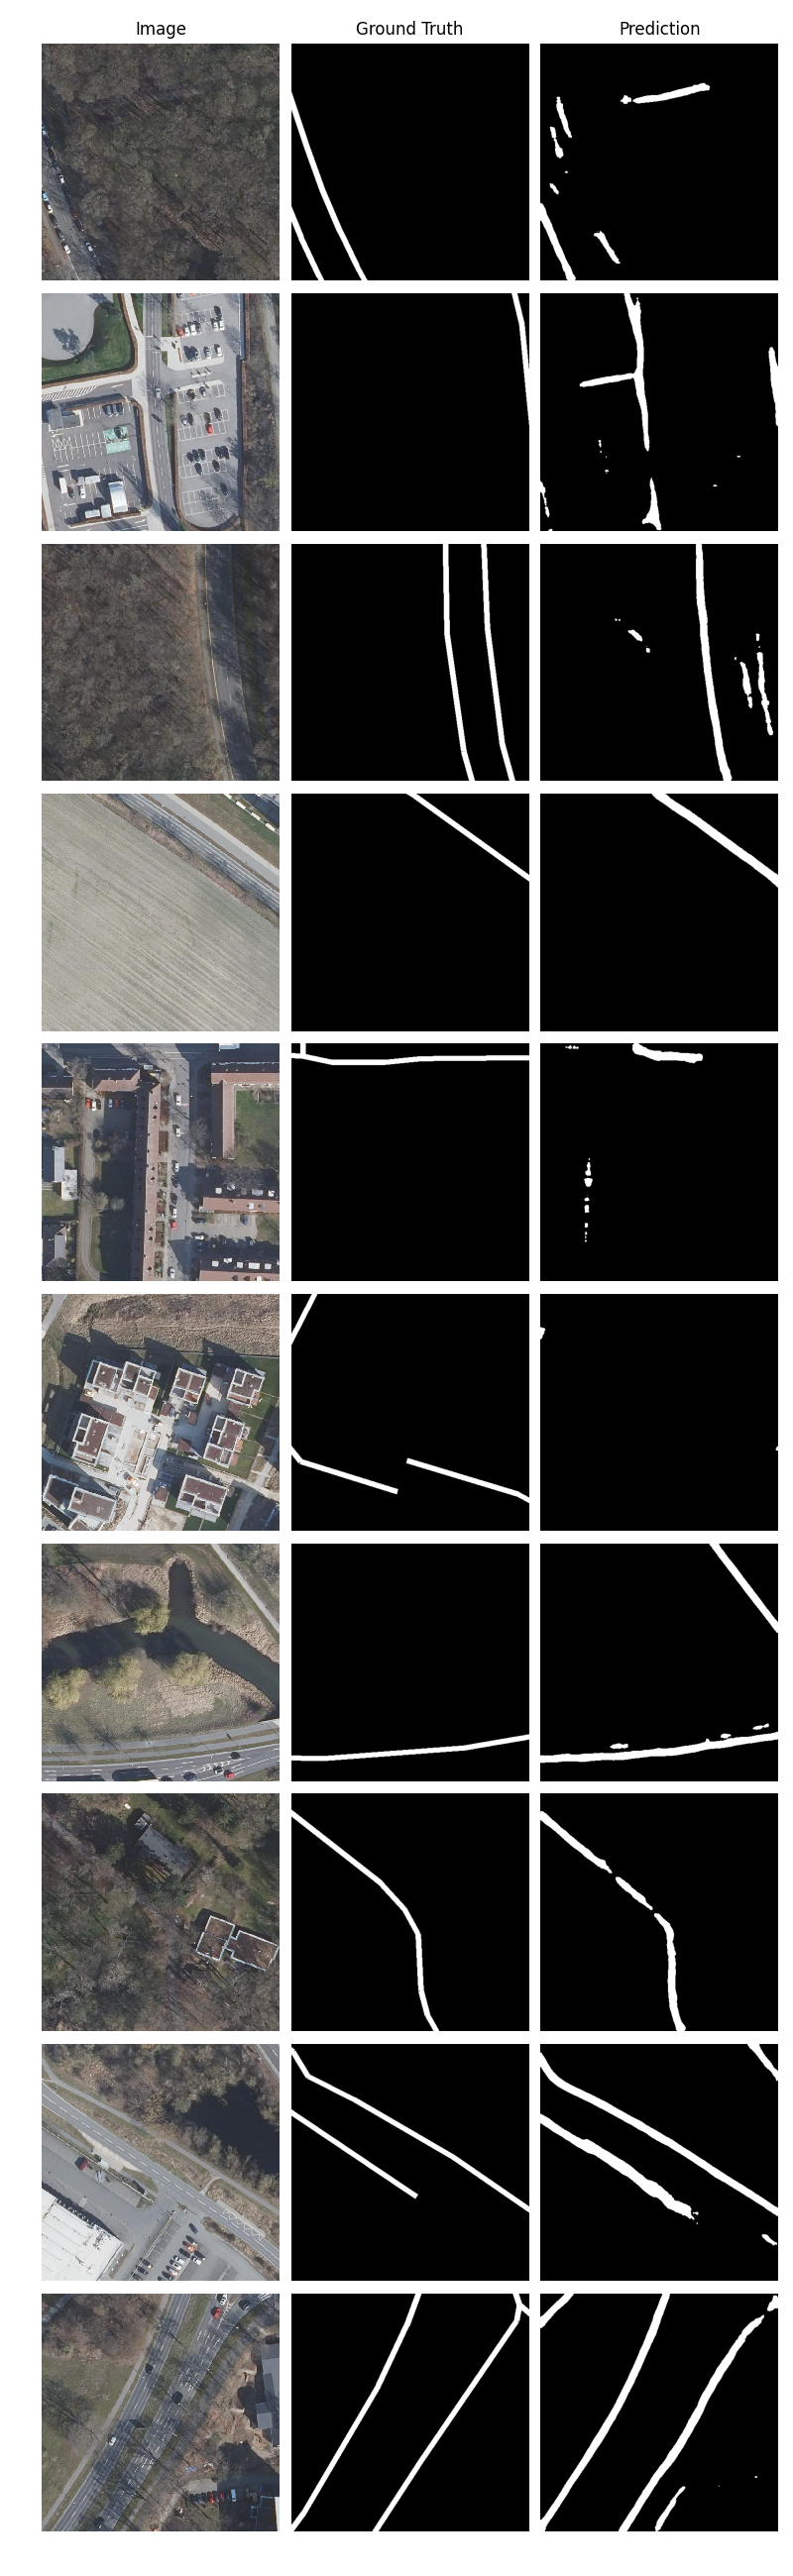
\includegraphics[width=1.\linewidth]{Bilder/Samples-Bikesat/bunet2-s.png}
		\caption{}
	\end{subfigure}
	\begin{subfigure}{.4\textwidth}
		\centering
		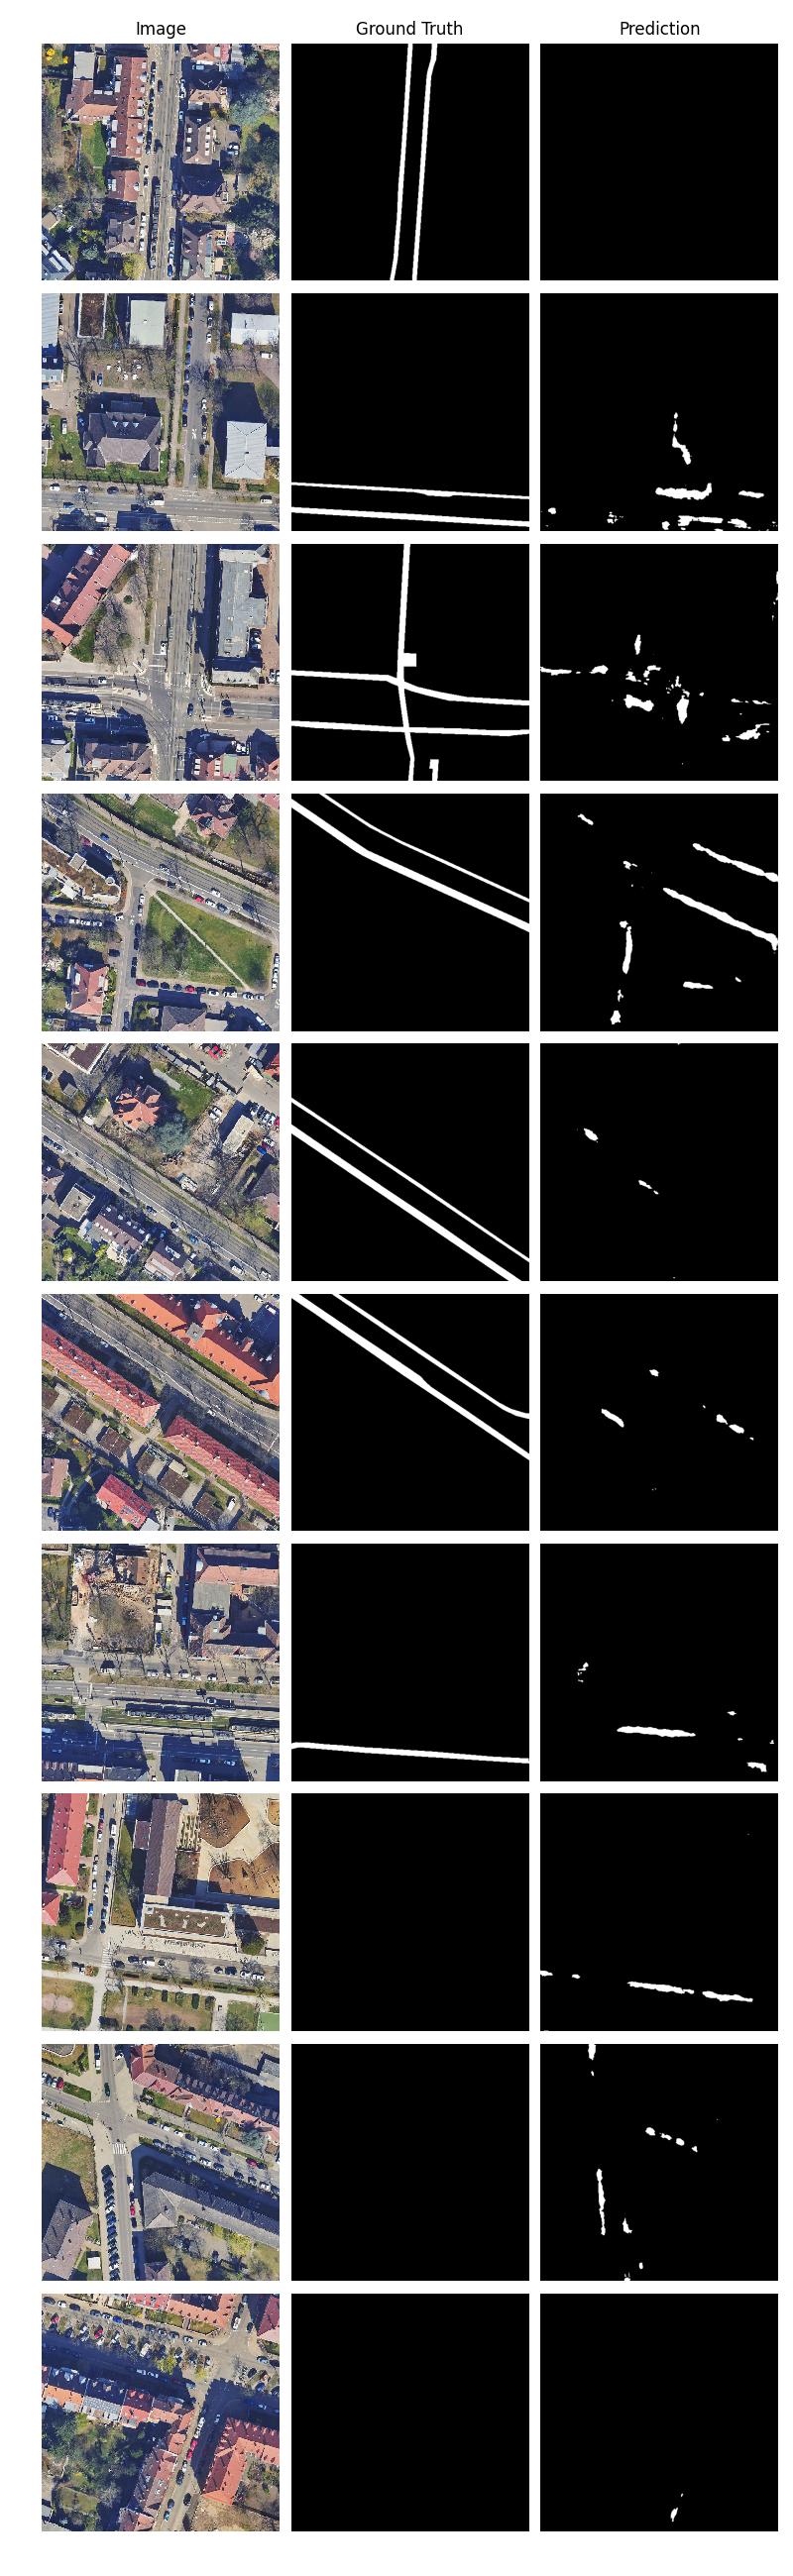
\includegraphics[width=1.\linewidth]{Bilder/Samples-Bikesat/vbunet-l.png}
		\caption{}
	\end{subfigure}

	\caption{Beispiel-Predictions des $BUNet2^*$ (a) und $VBUNet^l$ (b) auf dem BikeSat-Datensatz trainiert mit \textit{Basic}-Augmentation.}
	\label{fig:bikesat-samples-bunet2-s-vbunet-l}
\end{figure}

\begin{figure}[h]
	\centering
	\begin{subfigure}{.4\textwidth}
		\centering
		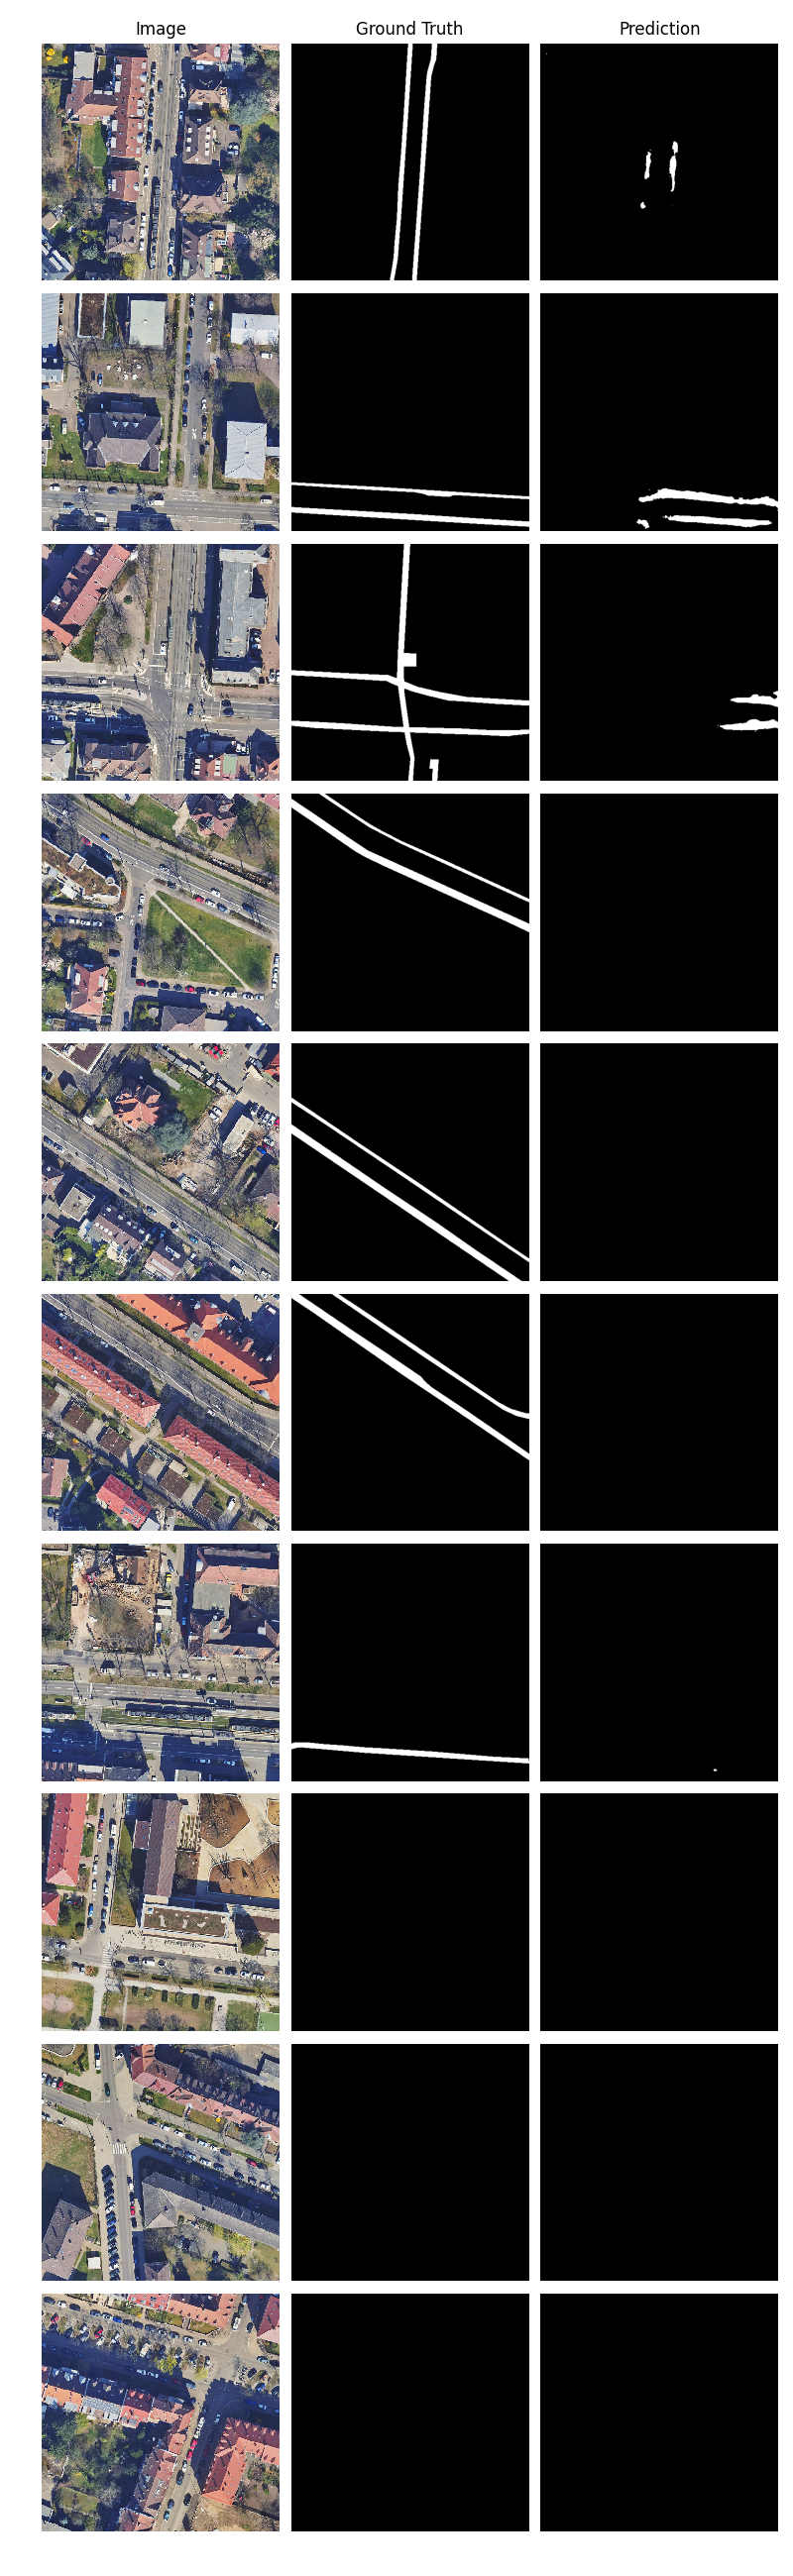
\includegraphics[width=1.\linewidth]{Bilder/Samples-KA/rbunet-l.png}
		\caption{}
	\end{subfigure}
	\begin{subfigure}{.4\textwidth}
		\centering
		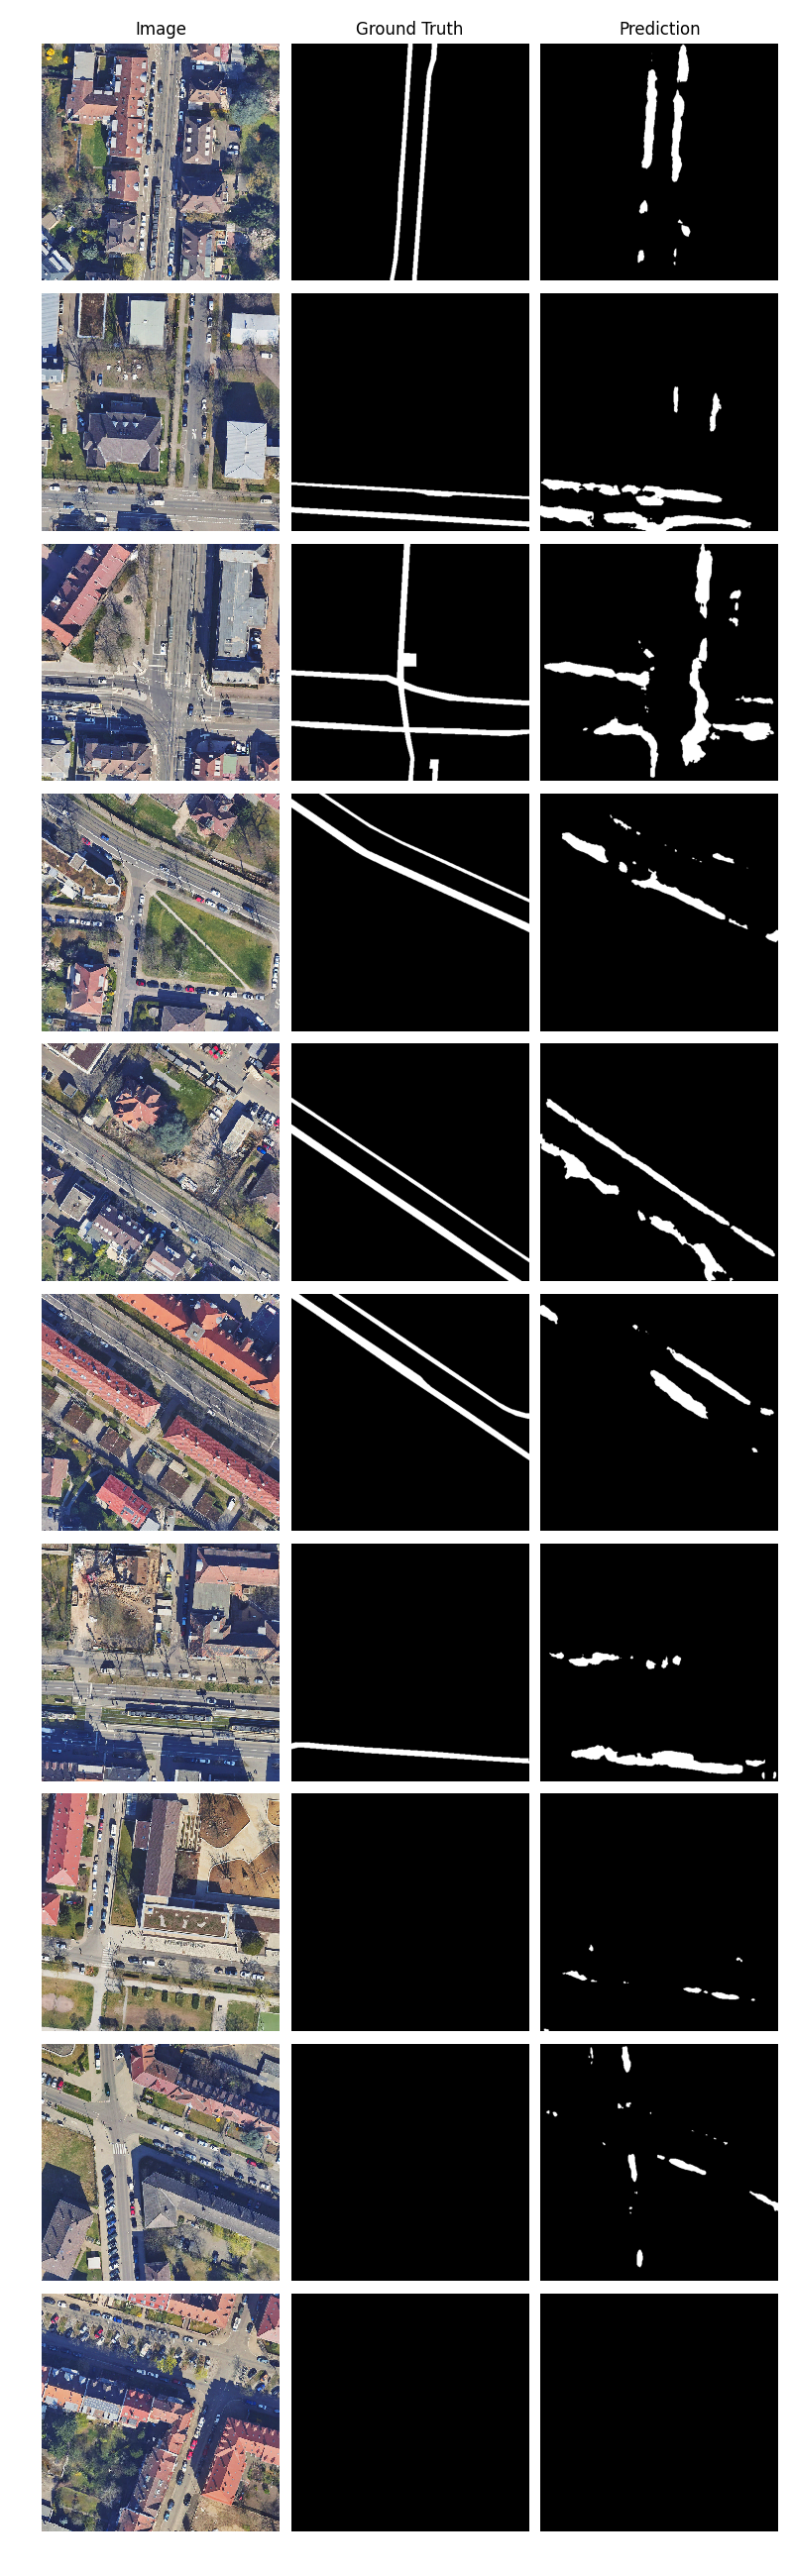
\includegraphics[width=1.\linewidth]{Bilder/Samples-KA/rbunet-s.png}
		\caption{}
	\end{subfigure}

	\caption{Beispiel-Predictions des $RBUNet^l$ (a) und $RBUNet^*$ (b) auf dem Karlsruhe-Datensatz trainiert mit \textit{Basic}-Augmentation.}
	\label{fig:ka-samples-rbunet-l-rbunet-s}
\end{figure}


\begin{figure}[h]
	\centering
	\begin{subfigure}{.4\textwidth}
		\centering
		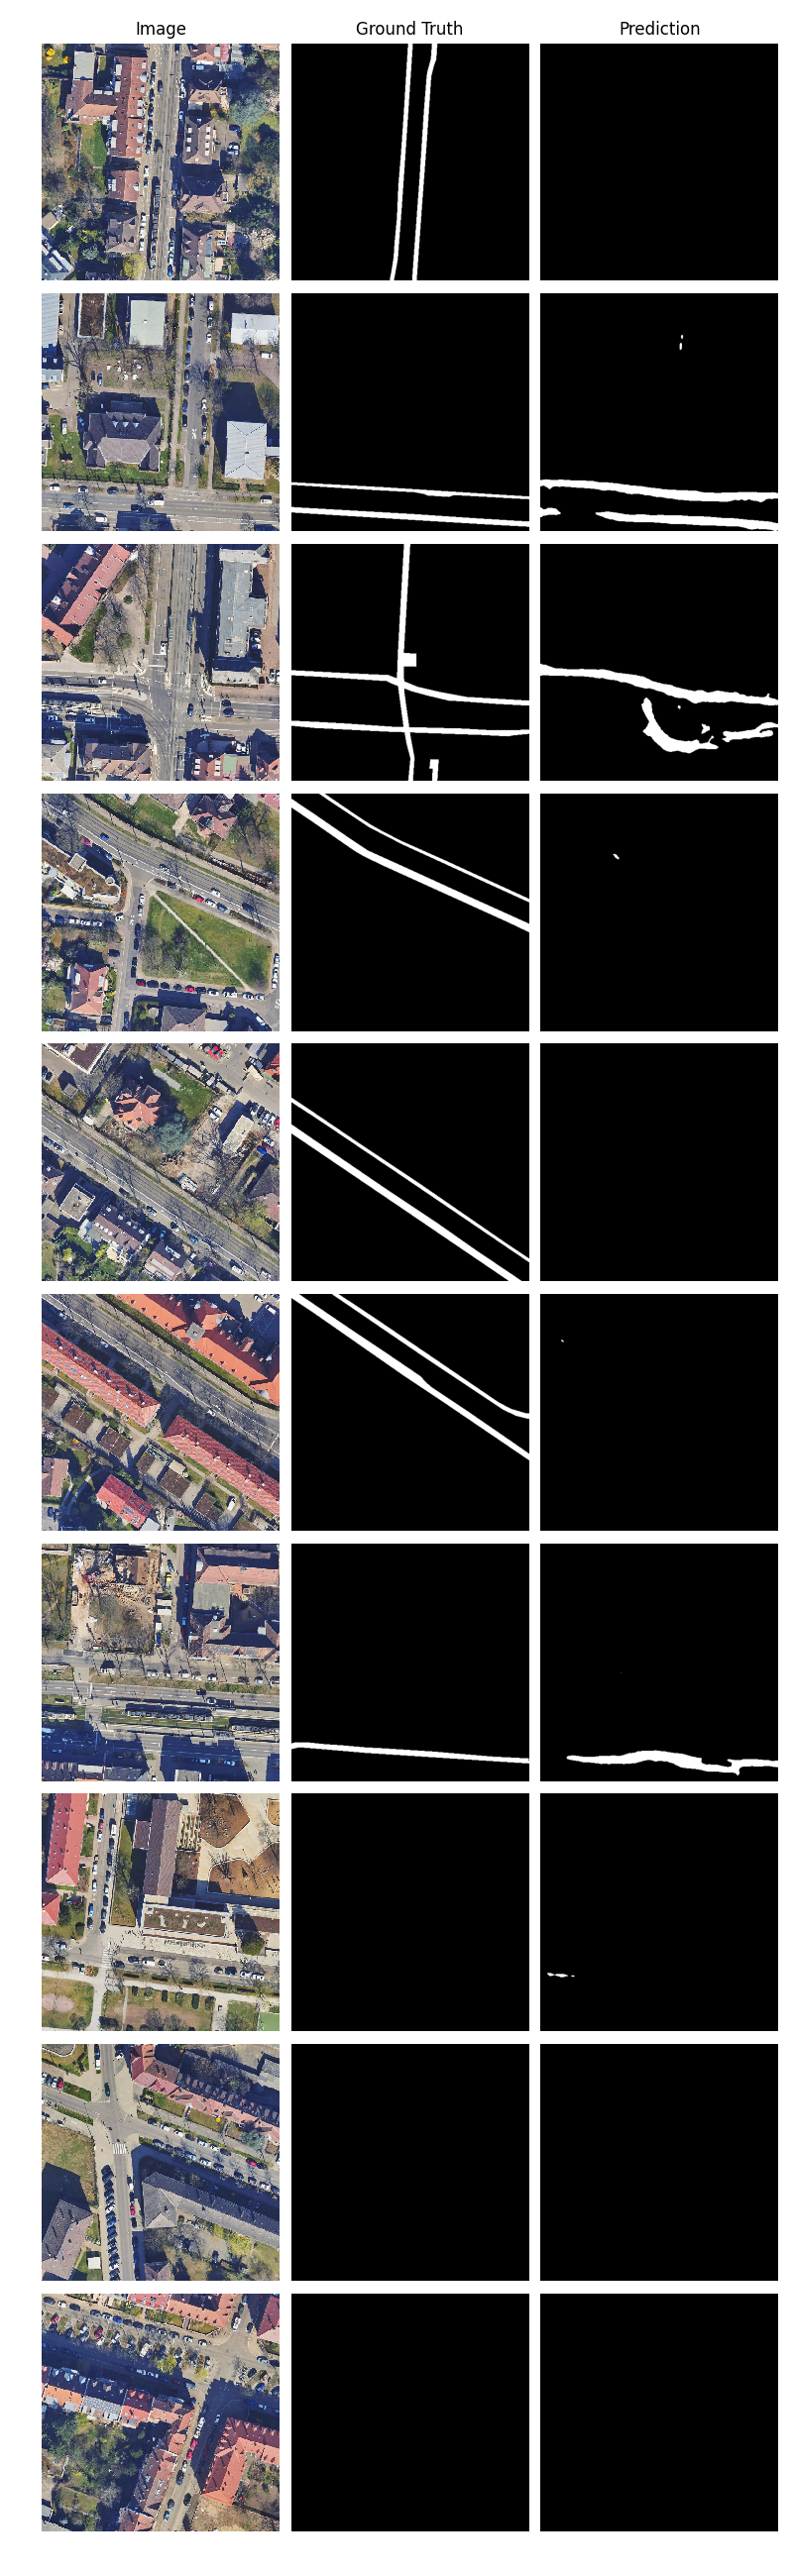
\includegraphics[width=1.\textwidth]{Bilder/karlsruhe-color-samples/rbunet-l.png}
		\caption{}
	\end{subfigure}
	\begin{subfigure}{.4\textwidth}
		\centering
		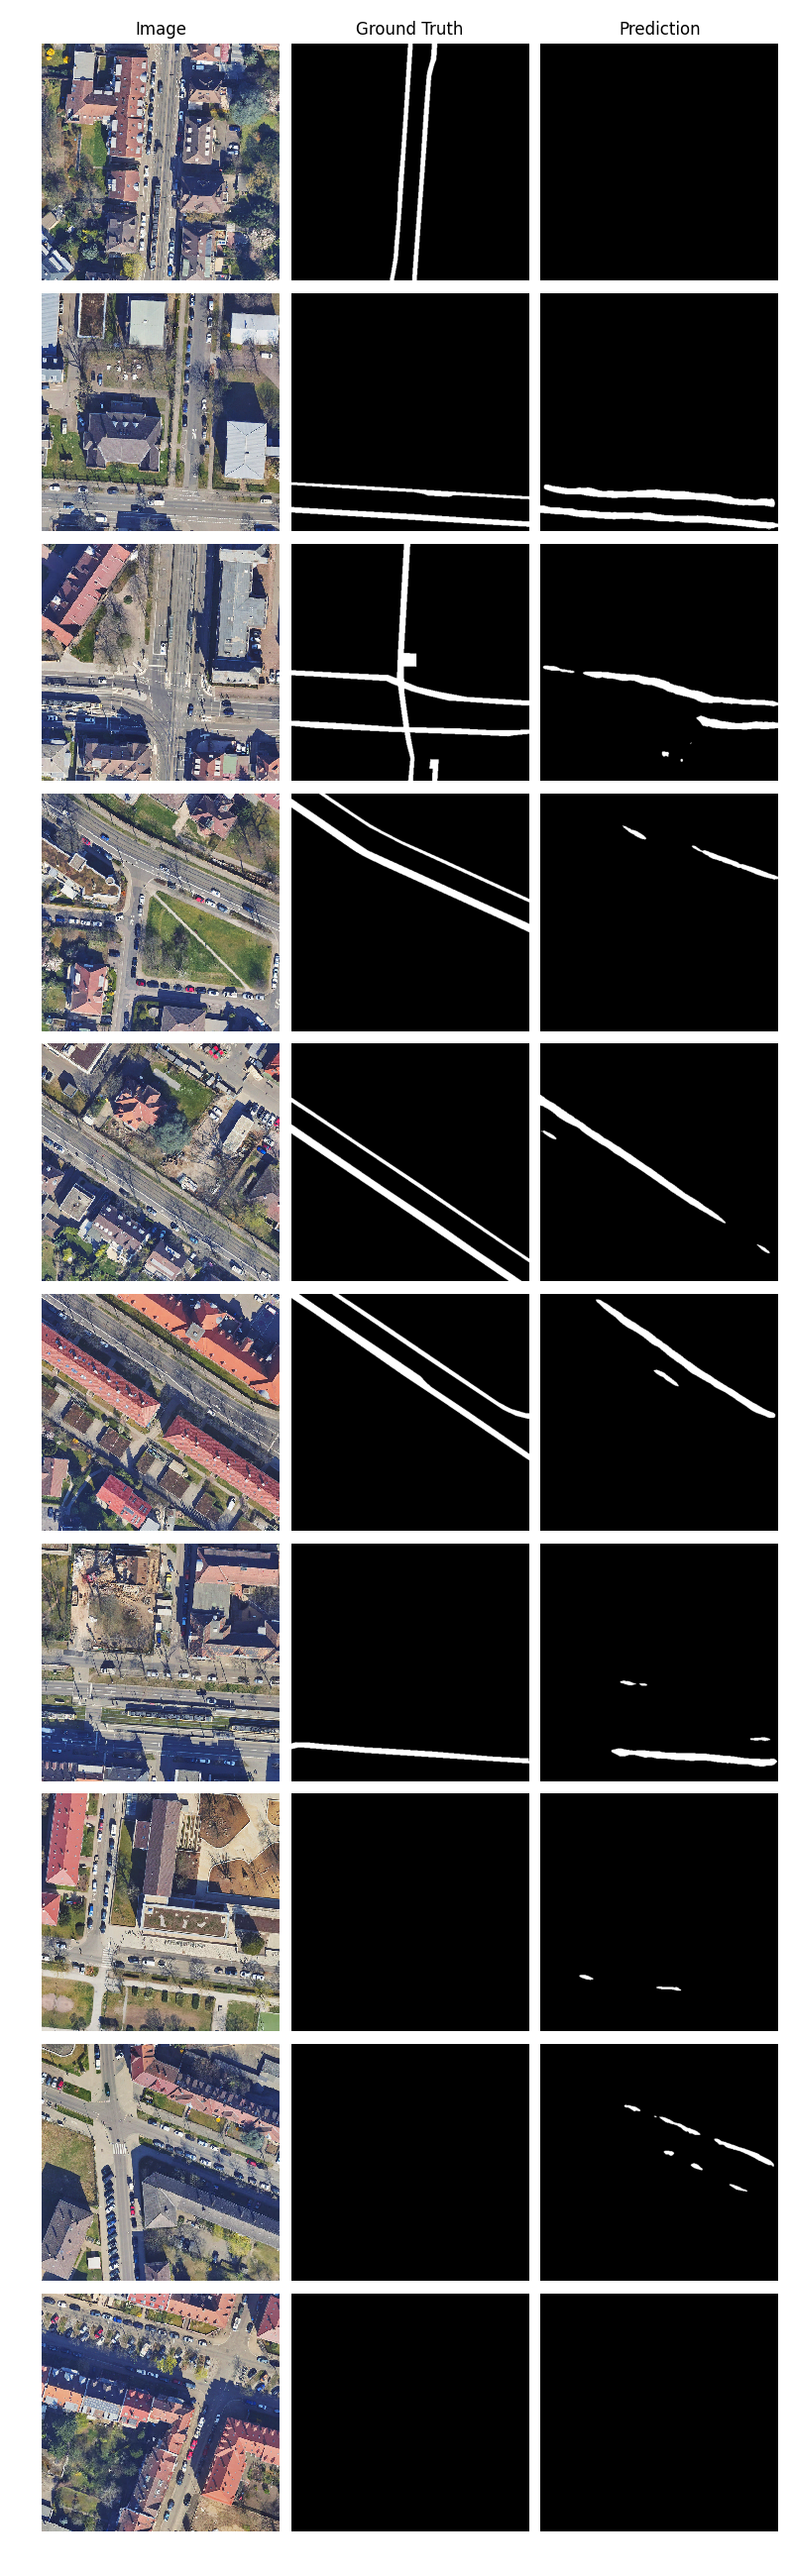
\includegraphics[width=1.\textwidth]{Bilder/karlsruhe-color-samples/rbunet-s.png}
		\caption{}
	\end{subfigure}
	\caption{Beispiel-Predictions des $RBUNet^l$ (a) und $RBUNet^*$ (b) auf dem Karlsruhe-Datensatz trainiert mit \textit{Color}-Augmentation.}
	\label{fig:ka-samples-rbunet-l-rbunet-s-color}
\end{figure}


\begin{figure}[h]
	\centering
	\begin{subfigure}{.4\textwidth}
		\centering
		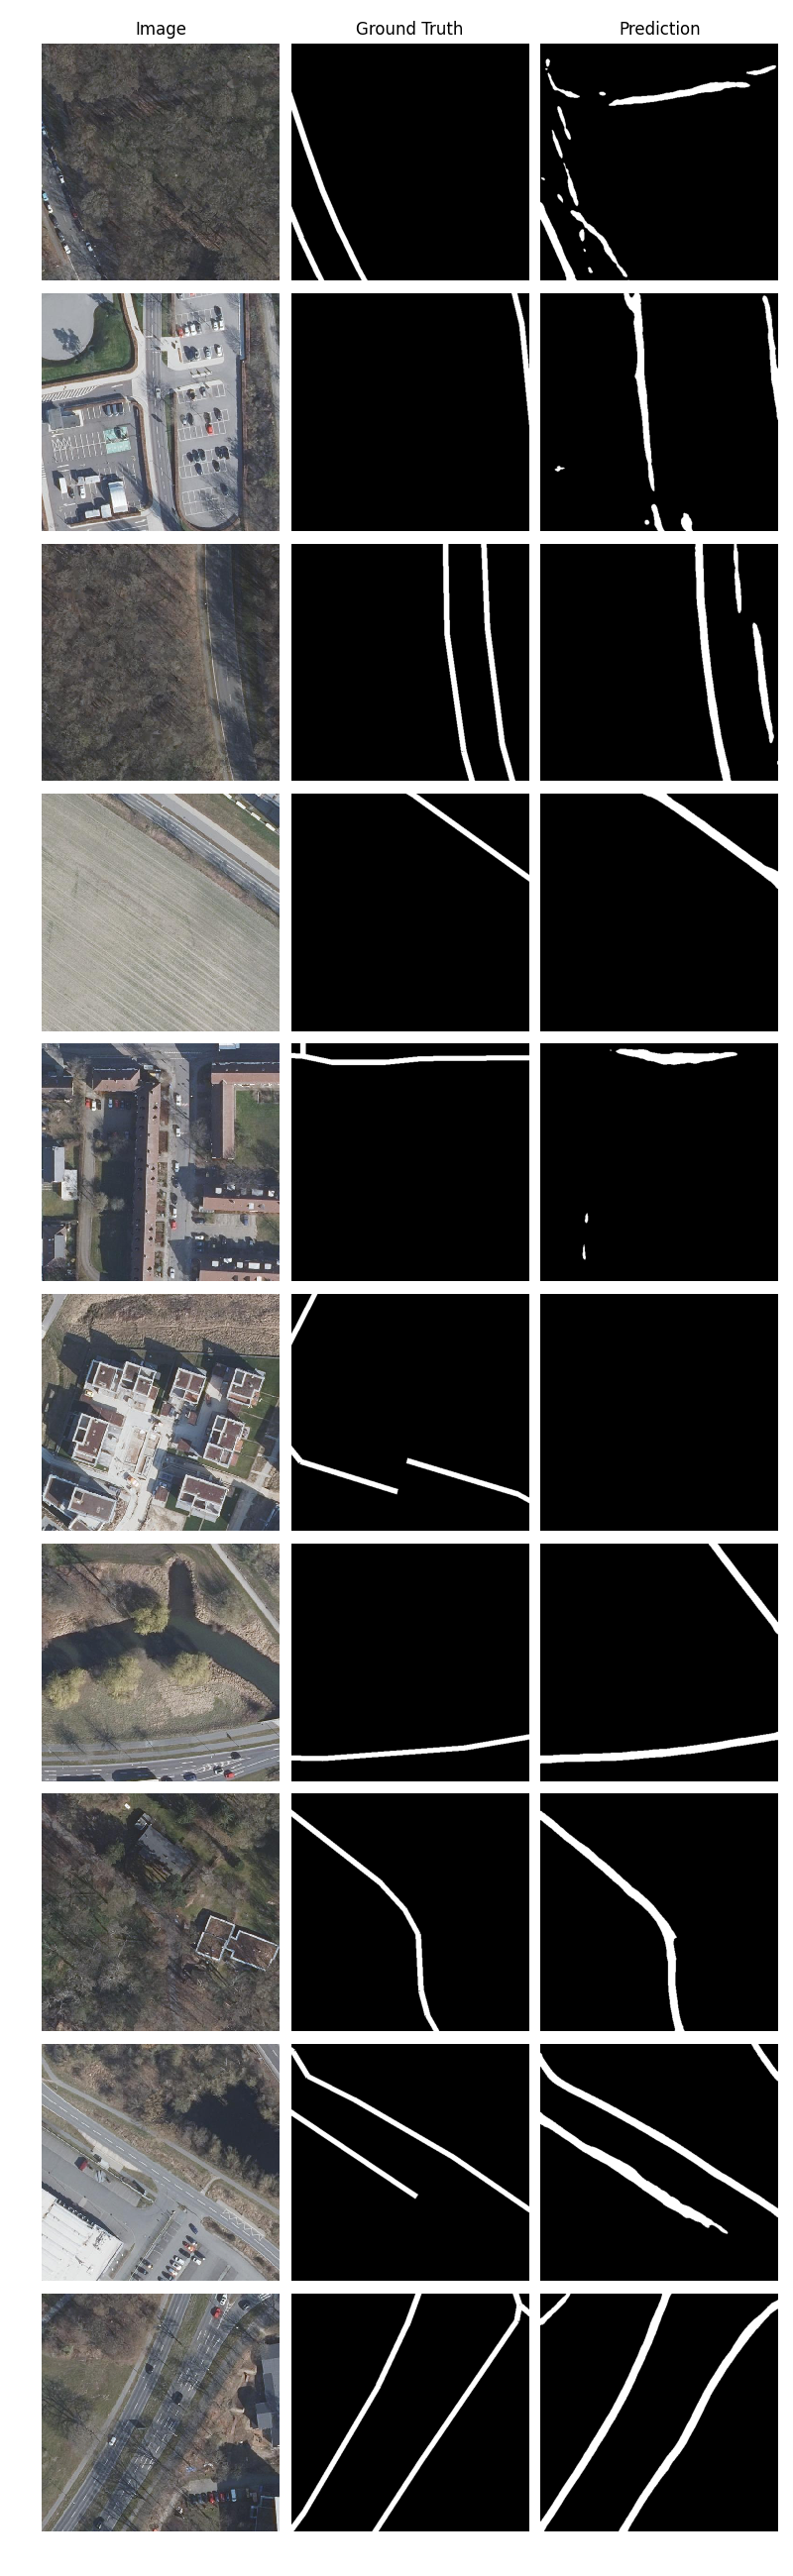
\includegraphics[width=1.\textwidth]{Bilder/wolfsburg-color-samples/rbunet-l.png}
		\caption{}
	\end{subfigure}
	\begin{subfigure}{.4\textwidth}
		\centering
		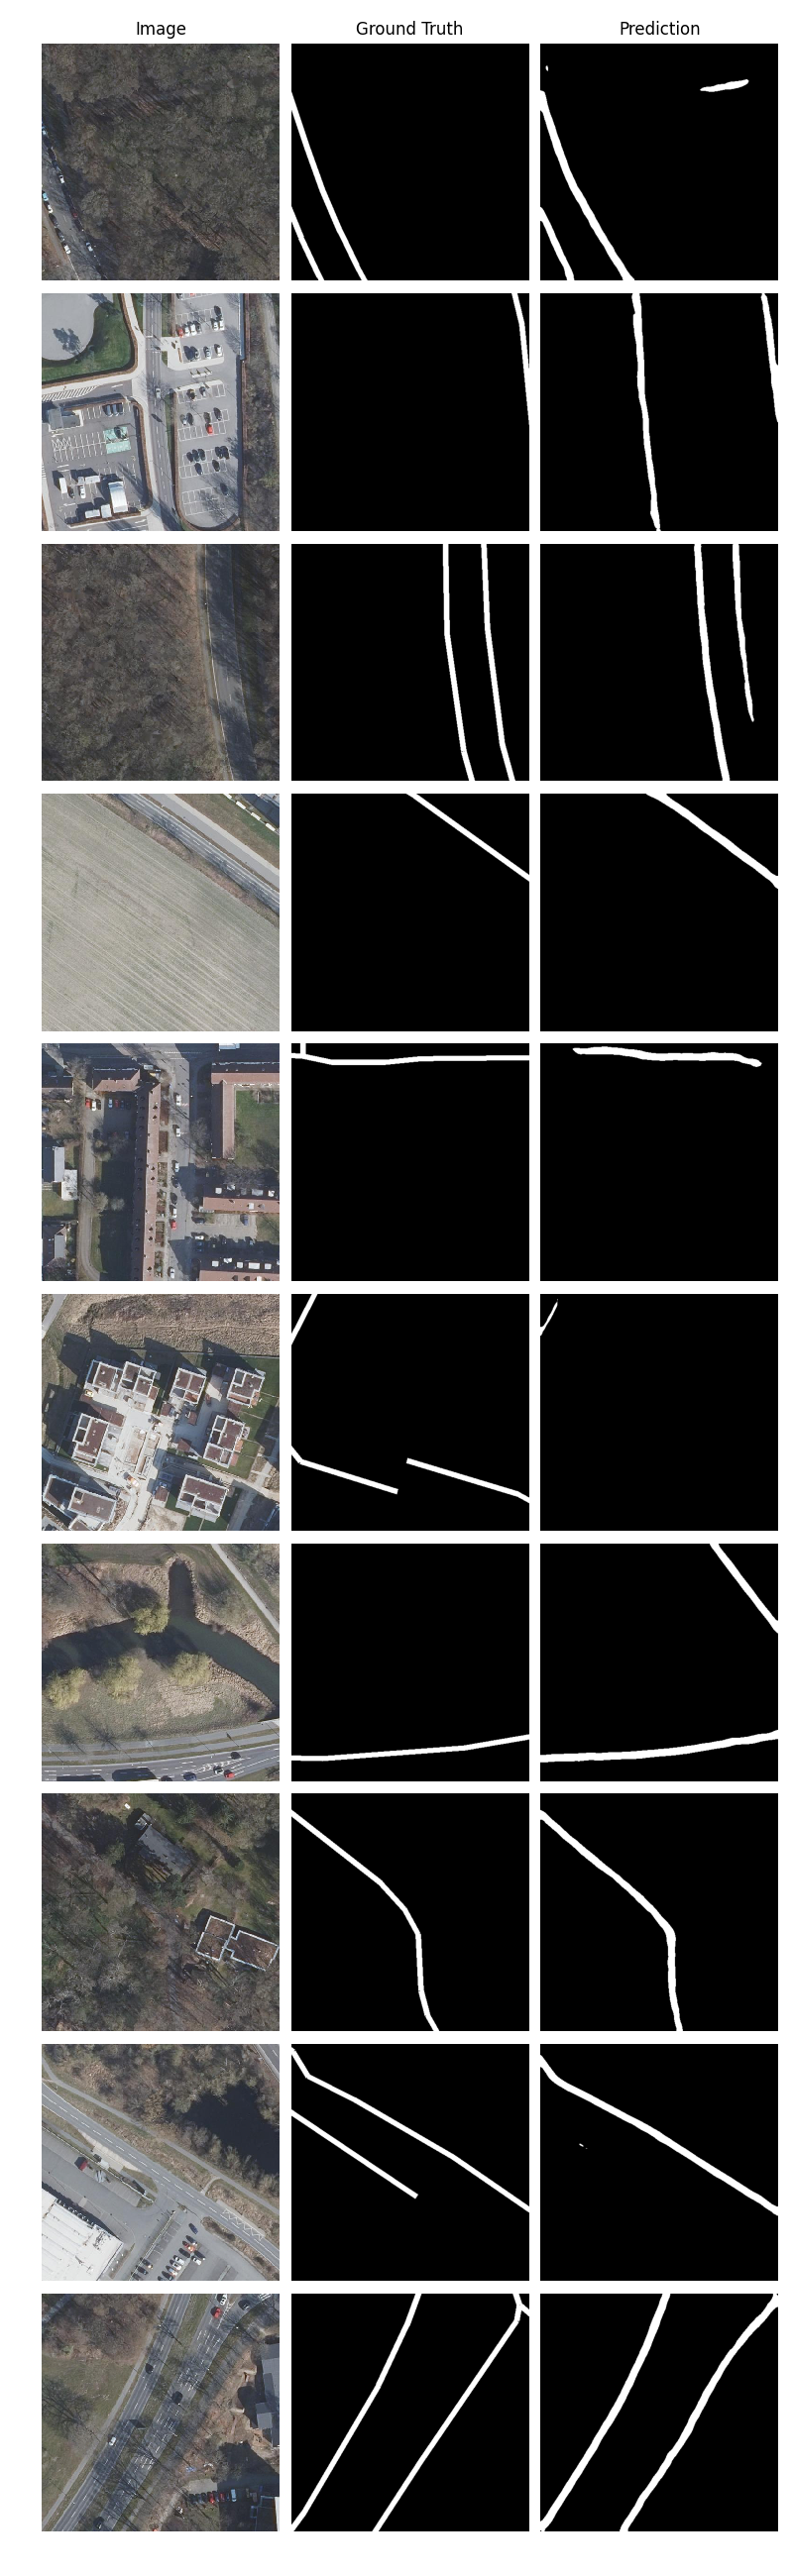
\includegraphics[width=1.\textwidth]{Bilder/wolfsburg-color-samples/rbunet-s.png}
		\caption{}
	\end{subfigure}
	\caption{Beispiel-Predictions des $RBUNet^l$ (a) und $RBUNet^*$ (b) auf dem Wolfsburg-Datensatz trainiert mit \textit{Color}-Augmentation.}
	\label{fig:wolfsburg-samples-rbunet-l-rbunet-s-color}
\end{figure}


\subsection{Ergebnisse auf gefiltertem Karlsruhe-Datensatz}

\begin{table}[ht]
	\centering
	\begin{tabular}{l|cc|cc}
		& \multicolumn{2}{c|}{Basic Aug.} & \multicolumn{2}{c}{Color Aug.} \\ 
		Modell & \ac{IoU} & \ac{BIoU}  & \ac{IoU} & \ac{BIoU}  \\
		\midrule
        BUNet2$^*$ & 02,78 & 07,31  &  14,19 & 27,43 \\
        BUNet2$^l$ & 04,23 & 09,90  &  15,15 & 29,35 \\
        BUNet2$^r$ & 01,94 & 04,67  &  10,45 & 21,33 \\
		\midrule

        BUNet15$^*$ & 07,85 & 17,12  &  16,72 & 37,16 \\
        BUNet15$^l$ & 05,59 & 10,17  &  19,11 & 42,00 \\
        BUNet15$^r$ & 04,94 & 10,06  &  16,41 & 33,52 \\
		\midrule

        VBUNet$^*$ & \underline{\textbf{23,80}} & \underline{\textbf{50,45}} &  \underline{\textbf{22,44}} & \underline{\textbf{47,20}} \\
        VBUNet$^l$ & 11,34 & 22,89 &  07,65 & 18,50 \\
        VBUNet$^r$ & \textbf{22,93} & 38,69 &  20,99 & 39,28 \\
		\midrule

        RBUNet$^*$ & \textbf{20,97} & \textbf{48,42} &  \textbf{21,12} & \textbf{46,11} \\
        RBUNet$^l$ & 04,62 & 08,19 &  18,76 & 34,47 \\
        RBUNet$^r$ & 11,58 & 20,49 &  14,93 & 27,59 \\
		\midrule

        DBUNet$^*$ & 17,52 & \textbf{43,53} &  20,82 & \textbf{45,16} \\
        DBUNet$^l$ & 09,73 & 25,43 &  18,74 & 32,97 \\
        DBUNet$^r$ & 19,77 & 36,33 &  \textbf{22,14} & 44,96 \\
        
	\end{tabular}
	\caption{Ergebnisse der Modelle auf dem Karlsruhe-Datensatz, wobei Bilder mit leeren Masken entfernt wurden. 
    In Prozent.}
	\label{tab:results-ka-small}
\end{table}

\autoref{tab:results-ka-small} zeigt die Test-Ergebnisse der Modelle aus \autoref{tab:results} 
auf allen 49 $512{\times}512$-Ausschnitten des Karlsruhe-Datensatz (s. \autoref{sec:karlsruhe}), 
\textit{die Radwegen enthalten}, in Prozent. 
Ein Ausschnitt enthält einen Radweg, wenn in der zugehörigen Label-Maske mindestens ein Pixel als Radweg annotiert ist. \\
Pro Spalte sind die höchsten drei Ergebnisse hervorgehoben und das höchste unterstrichen.
Die \ac{BIoU} hat eine Puffergröße von 15 Pixeln, wie in \autoref{sec:eval:biou} festgelegt.

\subsection{Ergebnisse bei fehlender Annotation}

Wie in \autoref{sec:bike-data} und \ref{sec:karlsruhe} beschrieben, wurde der BikeSat-Datensatz automatisch 
annotiert und der Karlsruhe-Datensatz von Menschen. Die Netze sind mit dem BikeSat-Datensatz trainiert. 
Wie bereits in \autoref{sec:bike-data} erwähnt, erhält die Datengrundlage zum BikeSat-Datensatz 
in einer von Menschen gesichteten und bewerteten Stichprobe \textbf{722} von \textbf{724} realen Radwegen.
Es fehlen also zwei Radwege. 

Die manuell von Menschen annotierten Bilder des Karlsruhe-Datensatzes zeigen dagegen eine höhere 
Fehlerquote. Die bestehenden Label sind zwar genauer platziert, aber dafür weniger vollständig. 
Hier ist bei einer Sichtung der Daten aufgefallen, dass ca. 15\% der Radwege nicht annotiert sind. 
Das hat aber keine Auswirkung auf das Training, da der Karlsruhe-Datensatz nur zum Testen verwendet wird.
\autoref{fig:annotation-mistake} zeigt ausgewählte Predictions (b)-(d) 
zu einem Ausschnitt aus dem Karlsruhe-Datensatz, bei dem bei der manuellen Annotation 
Radwege in der Straße, die von links unten nach rechts oben verläuft, übersehen wurden. 
In den Ausschnitten (c) und (d) sind die Radwege trotzdem erkannt, während es aber auch 
Beispiele wie (b) gibt, worin die querenden Radwege nicht getroffen sind. Ausschnitte (c) 
und (d) zeigen allerdings, dass die Netze Radwege erkennen können, die ein Mensch übersieht.
Es war allerdings kein Netz in der Lage für den gegebenen Bildausschnitt alle Radwege korrekt 
zu erkennen. \\
Was außerdem auffällig ist, ist, dass in Bild (c) der Radweg rechts unten genau getroffen ist 
(vgl. menschliche Annotation aus (a)), während in Bild (c) und (d) der Gehweg neben dem eigentlichen 
Radweg annotiert ist. Zudem fällt in (d) ein grober Fehler des Netzes auf, da hier klar Teile des 
blauen Dachs auf der rechten Bildseite annotiert sind.

\begin{figure}
	\centering
	\begin{subfigure}{.45\textwidth}
		\centering
		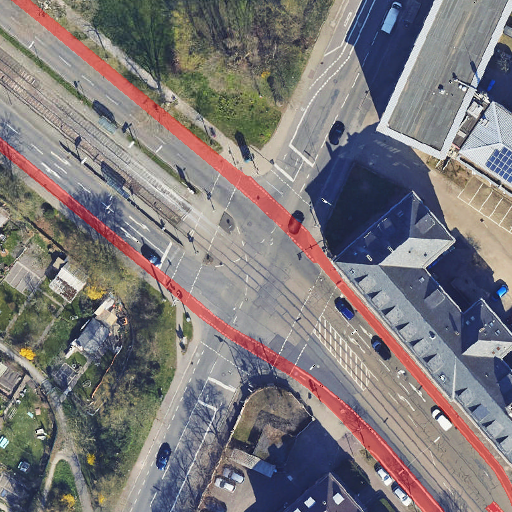
\includegraphics[width=1.\linewidth]{Bilder/annotation-mistake/overlayed.png}
		\caption{}
	\end{subfigure}
	\begin{subfigure}{.45\textwidth}
		\centering
		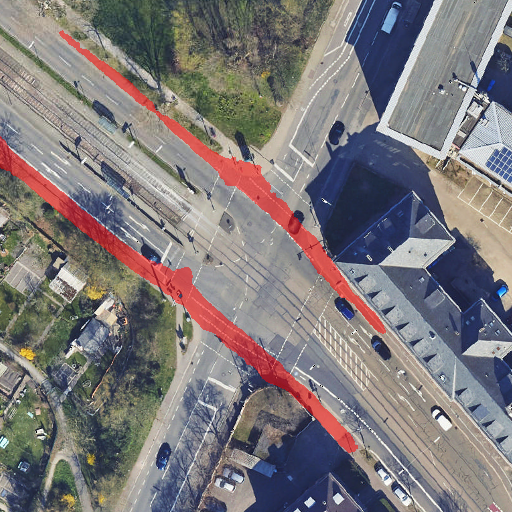
\includegraphics[width=1.\linewidth]{Bilder/annotation-mistake/straight-dbunet-r.png}
		\caption{}
	\end{subfigure} 
	\begin{subfigure}{.45\textwidth}
		\centering
		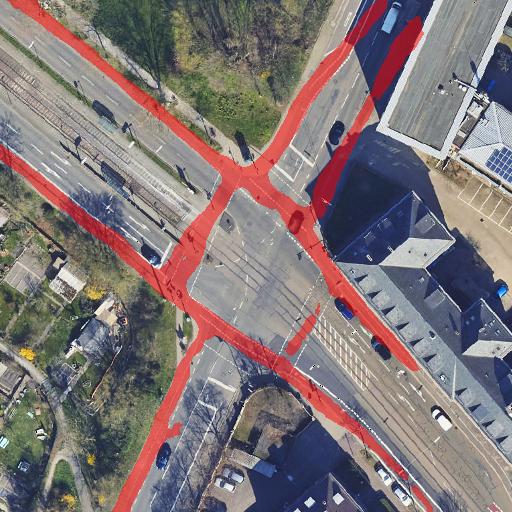
\includegraphics[width=1.\linewidth]{Bilder/annotation-mistake/fitting-vbunet-r.png}
		\caption{}
	\end{subfigure}
	\begin{subfigure}{.45\textwidth}
		\centering
		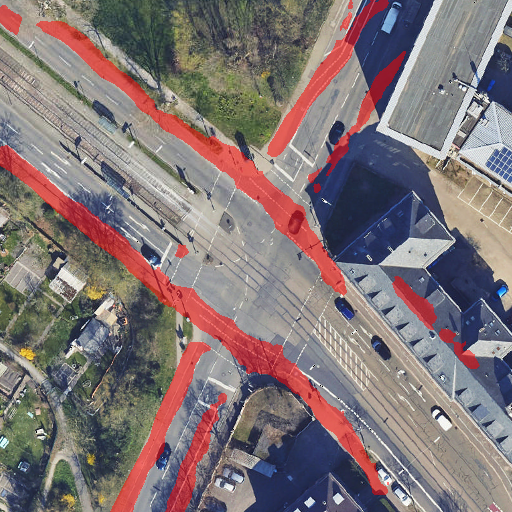
\includegraphics[width=1.\linewidth]{Bilder/annotation-mistake/full-vbunet-s.png}
		\caption{}
	\end{subfigure}

	\caption{(a) zeigt ein manuell annotierten Ausschnitt aus dem Karlsruhe-Datensatz, wobei Radwege 
	fälschlicherweise nicht annotiert sind. Abbildungen (b), (c) und (d) zeigen die Predictions von \ac{DBUNet}$^r$,
	\ac{VBUNet}$^r$, bzw. \ac{VBUNet}$^*$.}
	\label{fig:annotation-mistake}
\end{figure}

% networks tested with karlsruhe test data set  

% testing ./../Models/Double-Data\backbones\bike_mapper_pre-train-scratch-densenet121_Aug_IoU3076_q6178.h5
% iou: 0.07135618478059769, quality:0.45967867970466614

% testing ./../Models/Double-Data\backbones\bike_mapper_pre-train-scratch-resnet34_Aug_IoU2911_q6053.h5
% iou: 0.11737822741270065, quality:0.3280484974384308

% testing ./../Models/Double-Data\backbones\bike_mapper_pre-train-scratch-vgg16_Aug_IoU3045_q6148.h5
% iou: 0.09694375097751617, quality:0.3783626854419708

% testing ./../Models/Double-Data\pre-train\bike_mapper_pre-train-freeze-left_Aug_IoU2448_q5177.h5
% iou: 0.020918812602758408, quality:0.1211065948009491

% testing ./../Models/Double-Data\pre-train\bike_mapper_pre-train-freeze-right_Aug_IoU2535_q5127.h5
% iou: 0.09364935010671616, quality:0.47571051120758057

% testing ./../Models/Double-Data\pre-train\bike_mapper_triple-param_pre-train-freeze-left_Aug_IoU2814_q5714.h5
% iou: 0.1647404581308365, quality:0.5417148470878601

% testing ./../Models/Double-Data\pre-train\bike_mapper_triple-param_pre-train-freeze-right_Aug_IoU2822_q5726.h5
% iou: 0.10167630761861801, quality:0.5381019115447998

% testing ./../Models/Double-Data\road-pre-trained-backbones\bike_mapper_pre-train-densenet121freeze-left_Aug_IoU3155_q6238.h5
% iou: 0.17469285428524017, quality:0.5520145893096924

% testing ./../Models/Double-Data\road-pre-trained-backbones\bike_mapper_pre-train-densenet121freeze-right_Aug_IoU3212_q6299.h5
% iou: 0.14031212031841278, quality:0.5172706246376038

% testing ./../Models/Double-Data\road-pre-trained-backbones\bike_mapper_pre-train-resnet34freeze-left_Aug_IoU3098_q6051.h5
% iou: 0.24674279987812042, quality:0.6527144312858582

% testing ./../Models/Double-Data\road-pre-trained-backbones\bike_mapper_pre-train-resnet34freeze-right_Aug_IoU3131_q6355.h5
% iou: 0.18207795917987823, quality:0.5552724599838257

% testing ./../Models/Double-Data\road-pre-trained-backbones\bike_mapper_pre-train-vgg16freeze-left_Aug_IoU3224_q6293.h5
% iou: 0.12852726876735687, quality:0.5490880012512207

% testing ./../Models/Double-Data\road-pre-trained-backbones\bike_mapper_pre-train-vgg16freeze-right_Aug_IoU3184_q6151.h5
% iou: 0.175296351313591, quality:0.6151095628738403

% testing ./../Models/Double-Data\bike_mapper_scratch_Aug_IoU2354_q4771.h5
% iou: 0.013092363253235817, quality:0.3479517698287964

% testing ./../Models/Double-Data\bike_mapper_scratch_triple-param_Aug_IoU2793_q5655.h5
% iou: 0.21523651480674744, quality:0.5924956798553467

